\section{Proclivity for Physical Exercise - Before and After COVID-19}

\begin{figure}[h!]
	\centering
	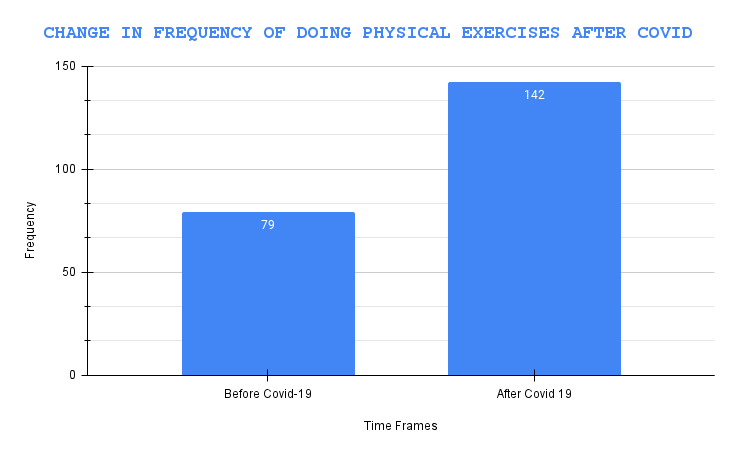
\includegraphics[width=0.9\linewidth]{IMAGES/Image 35.png}
	\caption{Physical Exercises after COVID-19}
	\label{G35}
\end{figure}

\ 

In the Bar diagram \ref{G35} illustrates findings from the aforementioned survey, showcasing the distinctions in physical exercise patterns before and after the onset of COVID-19. 

\

Based on the figure \ref{G35} depicting physical exercise frequency before and after COVID-19, it is evident that there was an increase in the frequency of physical exercise. Before COVID-19, the frequency was 79, while after COVID-19, the frequency rose to 142. This suggests a notable shift in exercise habits, with a higher number of individuals engaging in physical activities post-COVID-19 compared to the Pre-COVID-19 period. 

\

The increase in frequency may be attributed to various factors, such as heightened awareness of health, changes in daily routines, or a greater emphasis on physical well
being in response to the pandemic. 

\section{Impact on people, After spreading usage of sanitizers}

\begin{figure}[h!]
	\centering
	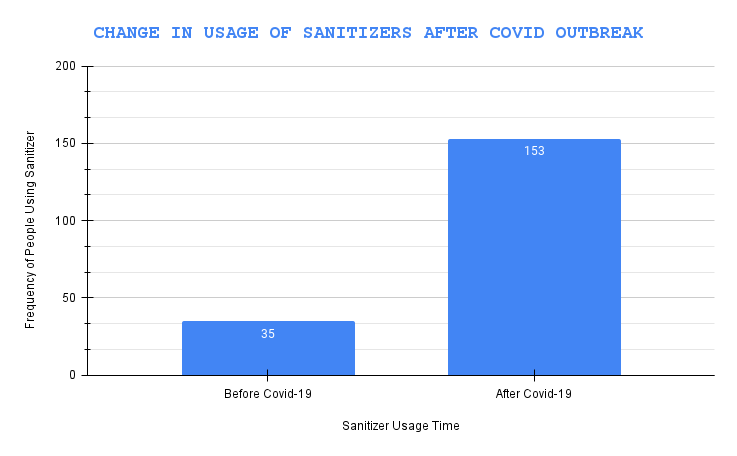
\includegraphics[width=0.9\linewidth]{IMAGES/Image 36.png}
	\caption{Sanitizer Usage}
	\label{G36}
\end{figure}

\ 

In the Bar diagram \ref{G36} represents the results of the above-mentioned survey, categorized by the Pre-COVID and Post-COVID usage of Sanitizers  

The diagram illustrates a significant change in the frequency of sanitizer usage time before and after COVID-19. Before the pandemic, the frequency of people using sanitizer was 35, whereas after COVID-19, this frequency increased substantially to 153. This considerable uptick in sanitizer usage suggests a heightened awareness and adherence to hygiene practices post-COVID-19. 

\

The substantial increase in frequency may be indicative of a broader societal shift towards prioritizing preventive measures for health and safety in response to the pandemic.

\section{Financial Coping Skills, A lesson of the Past : that shattered economy}

\begin{figure}[h!]
	\centering
	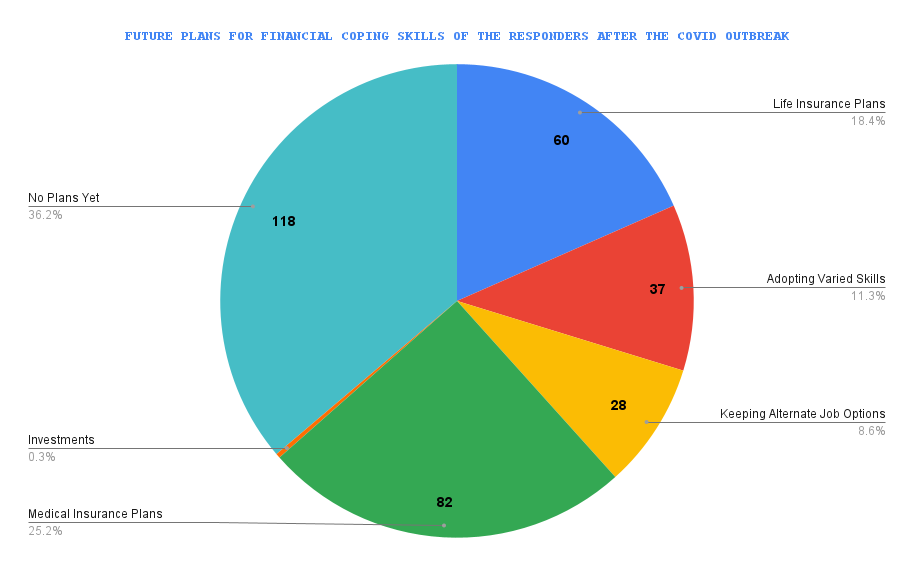
\includegraphics[width=0.9\linewidth]{IMAGES/Image 37.png}
	\caption{Financial Coping Skills}
	\label{G37}
\end{figure}

\ 

The Pie chart in \ref{G37} represents the distribution of Post-COVID financial coping strategies, with notable emphasis on medical insurance, varied skill acquisition, and a substantial portion undecided about future plans.

\

In summary, the analysis of post-COVID financial coping plans, as depicted in the chart, reveals a diverse landscape. Notably, 25.2\% of respondents prioritize their well-being with medical insurance, while 18.4\% consider life insurance. A proactive approach is evident, with 11.3\% aiming to acquire diverse skills, and 8.6\% exploring alternate job options. Surprisingly, only 0.3\% express plans for investments. Significantly, 36.2\% of individuals have yet to formalize specific financial strategies, underscoring the prevailing uncertainty. 

\

This numerical breakdown emphasizes the variety of approaches, highlighting the intricate and individualized nature of post-pandemic financial planning among surveyed individuals.

\section{Impact on general awareness in controlling a pandemic}

\begin{figure}[h!]
	\centering
	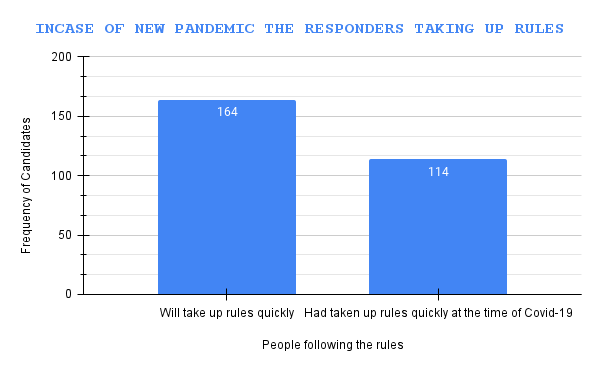
\includegraphics[width=0.9\linewidth]{IMAGES/Image 38.png}
	\caption{General awareness of public}
	\label{G38}
\end{figure}

\ 

As we can see from Figure \ref{G38} the harsh matter of fact, it is likely for the world to face more pandemics in the near future, followed by COVID-19. However a word of hope is that we have, from our data set, the number of people likely to follow government prescribed guidelines has increased quite a bit compared to that at the time of onset of COVID-19.

\

Out of $230$ individuals, the number $(114)$ of people, taking up guidelines and rules at the time of the Corona Outbreak is quite less than the number $(164)$ of people willing to quickly follow the new guidelines if a similar history of COVID repeats itself in near future. 

\

It is conclusive that a general awareness regarding the pandemic and its control have grown among the responders.